\section{Zarządca}
Zarządca jest elementem systemu odpowiedzialnym za komunikację z API zewnętrznego systemu STOS, przechowywanie plików zadań zdefiniowanych przez prowadzących zajęcia i plików rozwiązań dodanych do systemu przez studentów. Posiada również cache sprawdzający czy w plikach systemu znajdują się już pliki rozwiązania w celu optymalizacji ilości żądań wysyłanych do API.

\subsection{Implementacja}
Interfejs zarządcy został stworzony przy pomocy modułu Abstract Base Classes\cite{pythonAbc} i zawiera sygnatury trzech metod.
\lstset{style=python}
\begin{lstlisting}[caption = {Interfejs zarządcy.}]
    class IManager(ABC):

    @abstractmethod
    def listen(self) -> None:
        pass

    @abstractmethod
    def task_completion_callback(self, task_data: TaskData, output_path: Path) -> None:
        pass

    @abstractmethod
    def register_new_task_callback(self, callback: Callable[[TaskData], None]) -> None:
        pass
\end{lstlisting}
Funkcjonalność zarządcy jest realizowana przez klasy sterowników do komunikacji z API, przechowywania plików oraz cache, których metody są wywoływane w głównej pętli komponentu w metodzie \textit{listen} oraz przy wystąpieniu w systemie zdarzenia ukończenia sprawdzania zadania w metodzie \textit{task\_completion\_callback}.

\subsection{Przebieg pracy zarządcy}
Komponent ten pracuje w nieprzerwanej pętli, która kolejno synchronizuje stan lokalnej bazy zawierającej zadania zdefiniowane przez prowadzących zajęcia z bazą zewnętrznego systemu STOS-ui, sprawdza czy w zewnętrznym systemie znajdują się rozwiązania zadań oczekujące na sprawdzenie, pozyskuje ich pliki i informuje nasłuchujące komponenty o pojawieniu się nowego zadania oczekującego na sprawdzenie. Po wykonanej sekwencji wywoływana jest metoda \textit{sleep} pochodząca z modułu standardowej biblioteki Pythona \textit{time}\cite{pythonTime}, która zatrzymuje dalsze wykonanie pętli na czas zdefiniowany w pliku zawierającym zmienne środowiskowe systemu.
\lstset{style=python}
\begin{lstlisting}[caption = {Implementacja metody listen.}]
    @override
    def listen(self) -> None:
        self.__stos_logger.info("Starting manager process")
        while True:
            self.synchronize_filesdb()
            task_data = self._handle_task_download()
            self._notify_new_task(task_data)
            sleep(self.__request_timeout)
\end{lstlisting}
Poza wykonywaniem głównej pętli, zarządca nasłuchuje na zdarzenie ukończenia sprawdzania zadania. Przy wystąpieniu tego zdarzenia odsyła otrzymany rezultat zadania do zewnętrznego systemu STOS-ui oraz usuwa z systemu pliki powstałe w procesie kompilacji i oceny zadania.
\lstset{style=python}
\begin{lstlisting}[caption = {Implementacja metody wywoływanej przy zdarzeniu ukończenia sprawdzania zadania.}]
    @override
    def task_completion_callback(self, task_data: TaskData, output_path: Path) -> None:
        self.__stos_logger.info(f"Received task completion data for task {task_data.task_id}")
        self.__api_driver.upload_results(task_data.task_id)
        try:
            shutil.rmtree(output_path)
        except:
            self.__stos_logger.error(f"Error while deleting task {task_data.task_id} result directory")
\end{lstlisting}
\begin{figure}[!ht]
	\begin{center}
		\resizebox{1\textwidth}{!} {
			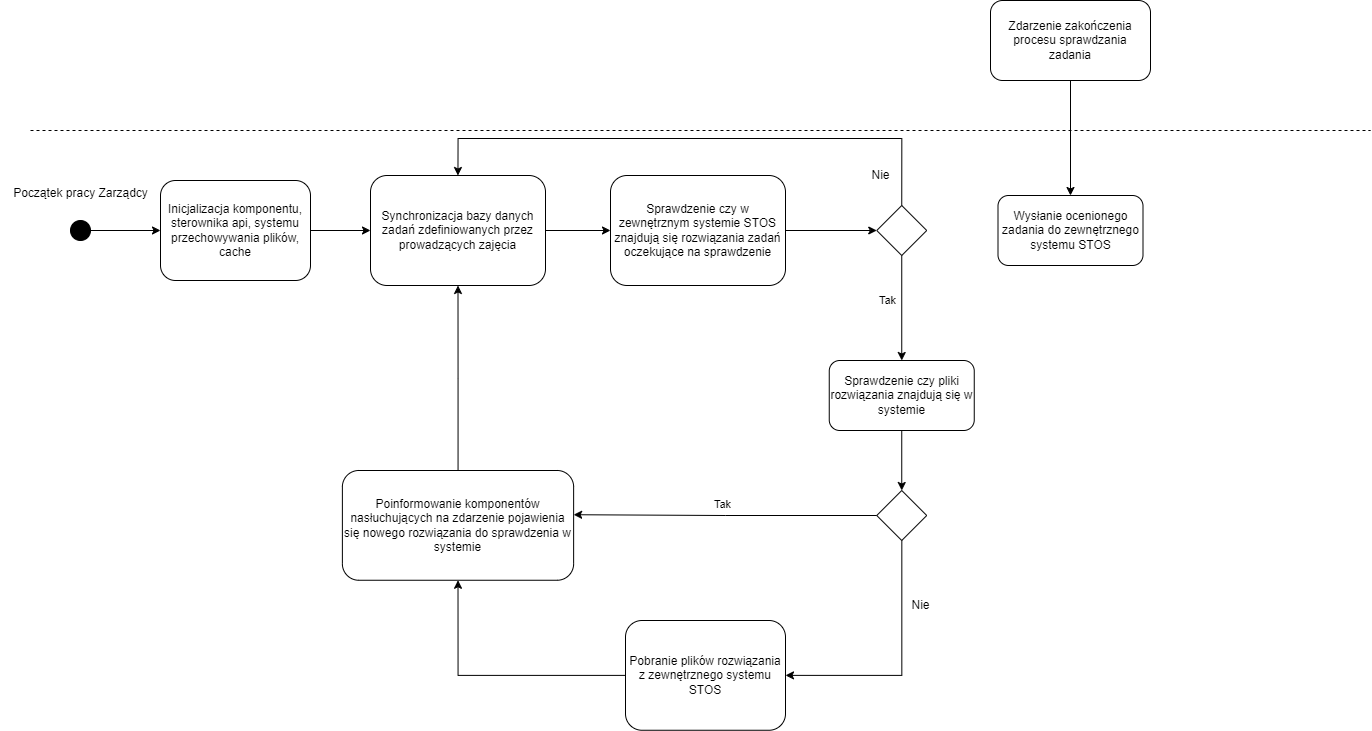
\includegraphics{img/3/zarzadca-diagram-aktywnosci.png}
		}
		\caption[Diagram aktywności zarządcy]{Diagram wizualizujący przebieg pracy zarządcy. Źródło własne.}
		\label{fig:scheduler-activity-diagram}
	\end{center}
\end{figure}

\subsection{Sterownik API}
Klasa sterownika API odpowiada za komunikację z zewnętrznym systemem STOS-ui poprzez żądania HTTP do udostępnianego przez niego API, obejmującego takie punkty końcowe jak:
\begin{itemize}
    \item \textit{GET /sync} - pobranie wartości skrótu bazy danych
    \item \textit{GET /sync\_problem} - pobranie pliku bazy danych
    \item \textit{GET /tasks} - pobranie listy zadań oczekujących na sprawdzenie
    \item \textit{GET /files/<file\_id>} - pobranie pliku źródłowego zadania o danym id
    \item \textit{POST /tasks/<task\_id>} - przesłanie rozwiązania zadania o danym id
\end{itemize}
Interfejs sterownika API zawiera sygnatury metod służących do odpytywania każdego z punktów końcowych udostępnianych przez STOS-ui.
\lstset{style=python}
\begin{lstlisting}[caption = {Interfejs sterownika API.}]
    class IApiDriver(ABC):

    # Downloads files of available task
    @staticmethod
    @abstractmethod
    def fetch_tasks() -> StosTaskResponse:
        pass

    # Downloads file of given id
    @staticmethod
    @abstractmethod
    def download_file(id: str) -> tuple[str, str]:
        pass

    # Uploads score of a given task
    @staticmethod
    @abstractmethod
    def upload_results(id: str) -> None:
        pass

    # Downloads hash of files.db database
    @staticmethod
    @abstractmethod
    def fetch_remote_tag() -> StosRemoteTagResponse: 
        pass

    # Downloads zipped files.db database
    @staticmethod
    @abstractmethod
    def fetch_filesdb_zip() -> None:
        pass
\end{lstlisting}
Żądania są wykonywane przy użyciu biblioteki requests\cite{pythonRequests}, która w znacznym stopniu upraszcza wysyłanie żądań HTTP w programach napisanych w języku Python.

\subsection{Sterownik systemu plików}
Interfejs sterownika systemu plików udostępnia dwie metody. Metoda \textit{save\_file} przyjmuje w argumentach nazwę, rozszerzenie oraz zawartość pliku i zapisuje go na dysku i zwraca ścieżkę do zapisanego pliku. Pliki zadań są potrzebne w systemie tylko na czas kompilacji i oceny, dlatego są zapisywane w folderze \textit{/tmp} przeznaczonym do przechowywania plików tymczasowych. Drugą metoda \textit{get\_file} służy do uzyskania zawartości pliku znajdującego się pod ścieżką podaną w argumencie metody.

\lstset{style=python}
\begin{lstlisting}[caption = {Interfejs sterownika systemu plików.}]
    class IStorageDriver(ABC):
    
    # Save file with filename and extension and return URL/PATH
    @staticmethod
    @abstractmethod
    def save_file(filename: str, content: str, extension: str) -> str:
        pass

    # Get contents of file under url. Returns None if file does not exist
    @staticmethod
    @abstractmethod
    def get_file(url: str) -> str | None:
        pass
\end{lstlisting}

\subsection{Sterownik cache}
Sterownik cache to element systemu mający zepewnić redukcję ilości wysyłanych żądań do systemu STOS-ui, poprzez przechowywanie plików wchodzących w skład zadania, dzięki czemu po uzyskaniu listy plików zadań, pobierane są tylko te, które nie znajdują się obecnie w cache. Sam cache został zaimplementowany przy wykorzystaniu bazy danych SQLite\cite{sqlite}, czyli bazy danych przeprowadzającej operacje zapisu i odczytu bezpośrednio na pliku na dysku, bez wykorzystywania dodatkowych procesów serwera bazy danych. Rozwiązanie to zostało wybrane ze względu na jego prostotę oraz fakt, że jest to baza danych wykorzystywana w innych miejscach systemu. Interfejs sterownika cache udostępnia metody do dodawania, usuwania i pobierania plików oraz metodę \textit{check\_files}, która w argumencie przyjmuję listę nazw plików. Metoda ta sprawdza, czy w cache znajdują się pliki, których nazwy znajdują się na liście i zwraca listę z nawami tych, których brakuje.
\lstset{style=python}
\begin{lstlisting}[caption = {Interfejs sterownika systemu plików.}]
    class ICacheDriver(ABC):

    # Checks cache for existence of files and returns missing files
    @staticmethod
    @abstractmethod
    def check_files(files: list[str]) -> list[str]:
        pass

    # Adds entry regarding a single file to cache and overwrites old record
    @staticmethod
    @abstractmethod
    def add_entry(file: str, path: str) -> None:
        pass

    # Deletes a record representing file
    @staticmethod
    @abstractmethod
    def delete_entry(file: str) -> None:
        pass

    # Get file entry, returns None if file does not exist
    @staticmethod
    @abstractmethod
    def get_entry(file: str) -> TaskFile | None:
        pass
\end{lstlisting}

